\chapter{Porting Xen Network Virtualization\label{cha:chapter6}}
In this chapter, first Xen network virtualization architecture will be explained and then the work related to porting it to PHIDIAS will be presented. Other split drivers for different I/O devices can ported using the same approach adopted for paravirtualized network driver with some little modifications corresponding to the requirements for these split drivers.

\section{Xen Network Virtualization \label{sec:xennetwork}}
In this section, analysis of xen network virtualization architecture and data flow will be provided. The details of bringing up network virtual interfaces in domains will be explained. Most of the steps performed during registration and initialization of xen network drivers also applies to other I/O virtual drivers of xen. Figure \ref{xennet_arch} shows basic components of xen network virtualization architecture which are explained in next sections.
\begin{figure}[!htbp]
	\centering
	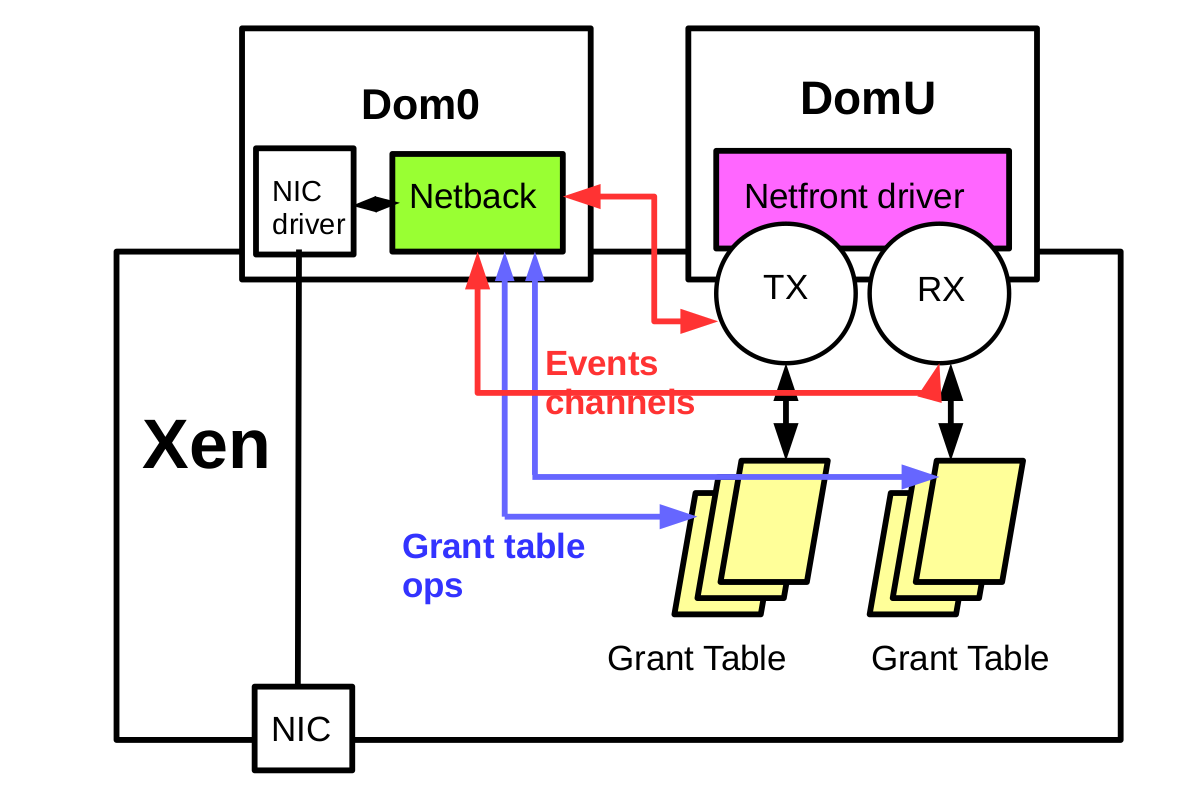
\includegraphics[width=10cm]{xennet_arch}
	\caption{Xen network virtualization architecture}
	\label{xennet_arch}
\end{figure}

\subsection{XenBus Backend and Frontend drivers \label{sec:xenbus}}
All split I/O drivers of Xen depends upon a general bus entity named XenBus which provides an interface to backend and frontend drivers to communicate with each other. The internal working of Xenbus is dependent upon Xenstore and event channels. Xenbus is also composed to two split drivers that work together to provide successful connection of I/O split drivers as shown in Figure \ref{xenbus_xs} .These are:
\begin{itemize}
	\item \textbf{XenBus Backend} is a bus that itself is registered with kernel bus subsystem. It is responsible for enumerating all backend devices in Xenstore, calling their corresponding probe functions and watching xenstore for changes. All backend drivers register themselves with XenBus backend.
	\item \textbf{XenBus Frontend} is also a type of bus which registers itself with kernel bus subsystem. It is responsible for enumerating and probing all frontend devices in Xenstore and registering watches in Xenstore for getting notification about changes in the backend devices. All frontend drivers registert themselves with XenBus frontend.
\end{itemize}
\begin{figure}[!htbp]
	\centering
	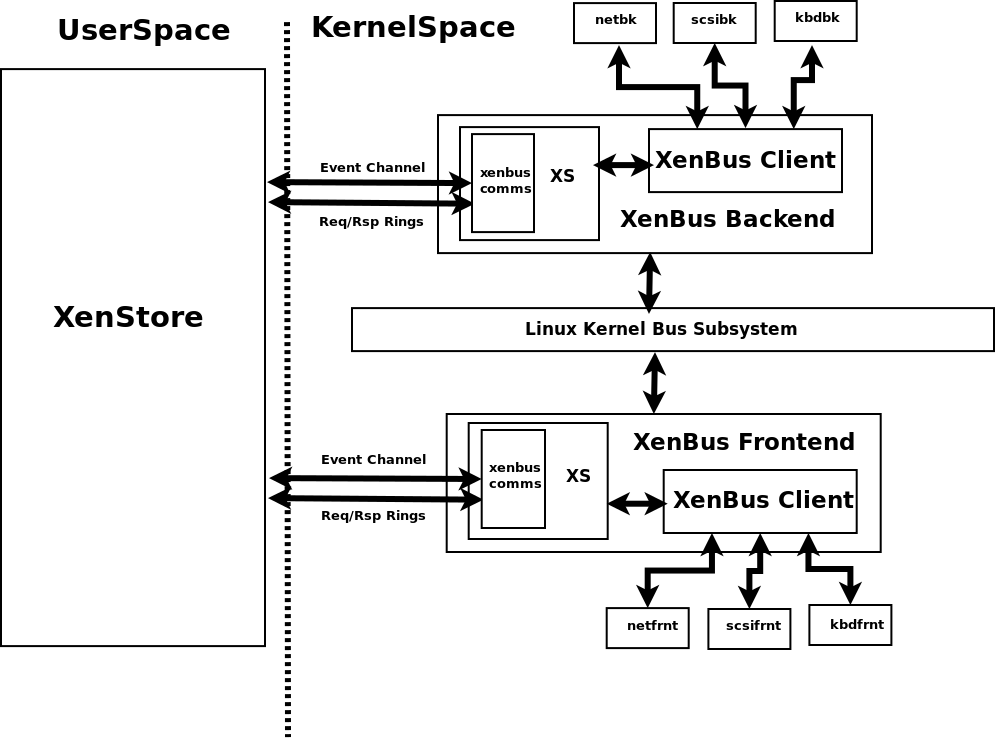
\includegraphics[width=10cm]{xenbus_xs}
	\caption{XenBus Architecture for connecting backends with frontends in Xen}
	\label{xenbus_xs}
\end{figure}

\subsection{Netback Driver \label{sec:netback}}
In Xen, Netback driver implements backend of split driver model in Dom0. It communicates with other end of split driver model through two rings i.e. transmit Tx ring and receive Rx ring. These rings are shared by network frontend driver and netback maps them into Dom0 address space. Netback driver is responsible for sending and receiving network packets to actual hardware through actual network driver of physical hardware. 

\subsection{Netfront Driver \label{sec:netfront}}
Netfront driver implements the frontend of split driver model in unprivileged domains. It creates Tx and Rx rings for sending instructions about data flow to the backend. These rings do not create actual data packets. The data packets are transferred using shared memory pages offered by grant table mechanism of Xen. Both frontend and backend notifies each other of requests and responses through event channel.

\subsection{Initialization of Network split drivers in Xen \label{sec:initnet}}
Netback driver is probed when Xend toolstack in Dom0 creates \textbf{`vif'} device. In this netback\_probe function, network backend sets its state to XenbusStateInitialising. It then write keys to the Xenstore related to features it supports for data processing. It includes feature-sg, feature-gso-tcpv4, feature-gso-tcpv6,feature-ipv6-csum-offload, feature-rx-copy,feature-rx-flip, feature-multicast-control, feature-dynamic-multicast-control,feature-split-event-channels, multi-queue-max-queues and feature-ctrl-ring. It then reads the main script provided in DomU XL configuration file for interfacing virtual network interface with real network device and kickoffs the necessary scripts to setup the desired connection between virtual interface and real network device. There are three main styles of network setup for a Xen host, bridged, routed and nat \cite{xen_network}. The default mode is bridged and from Xen 4.3 onwards, support of openvswitch is also provided.
\\
\\
Netfront driver gets probed by xenbus\_probe function during its initialization only if Xenstore is up and running.Netfront probe calls xennet\_create\_dev to create a net\_device and registers this device with Linux Network stack. It also allocates the transmit queue and receive queues for this net\_device. After DomU is started and netfront driver is initialized successfully, hotplug scripts in Dom0 sets the initial state of netfront to XenbusStateInitialising by writing corresponding netfront state key in Xenstore. Both netback and netfront has registered a notifier with Xenstore through Xenbus which watches the state of other end and get notifications from Xenstore upon changes in state of other end. Setting of the state of netfront to XenbusStateInitialising causes netback to get notified and it changes its Bus state to XenbusStateInitWait. When netfront driver gets notified about XenbusStateInitWait of netback, it calls xennet\_connect function. xennet\_connect is the main function which does all the necessary work to connect netfront with netback. It  creates tx and rx shared rings, grants the access right to netback, allocates tx and rx event channels and store tx-ring-ref, rx-ring-ref, event-channel-tx, event-channel-rx request-rx-copy, feature-rx-notify, feature-sg and feature-gso-tcpv4 to xenstore. It also allocates rx buffers for receiving packets from netback. After completing its talk with netback, it sets its state to XenbusStateConnected. 
\\
\\
On receiving state change notification about successful connection from netfront, netback reads the keys written by netfront. It reads grant refs of tx and rx rings and maps them into Dom0 address space. It binds its event channels to netfront tx and rx event channels. It then finally sets its state to XenbusStateConnected.


\subsection{Network Data Flow from Netfront to Netback \label{sec:tx}}
For transmitting network packets to netback, netfront calls xennet\_start\_xmit function. It examines received skb\_buff structure which is used by kernel to manage network packets. First, it allocates grant reference and tx request for linear part of skb\_buff. Then it calculates the number of fragments in network packet and allocates grant reference and tx request for all fragments of skb\_buff. Finally, it notifies netback driver of tx requests in Tx ring. 
\\
\\
On getting notification from netfront about tx requests, netback processes the requests in xenvif\_tx\_action and creates corresponding copy and map operations to be performed on shared grant references. Netback driver has the maximum length of TX copy operation to be 128 bytes. If the packet size is larger than 128 bytes, remaining data will be mapped into Dom0 address space. After filling a newly allocated skb\_buff with received network packet data, netback gives this packet to Linux network stack which forwards it to upper layers.

\subsection{Network Data Flow from Netback to Netfront \label{sec:rx}}
For transmission of packets from netback to netfront, xenvif\_start\_xmit is called. It first checks the number of available of rx buffer slots in RX ring of netfront mapped into Dom0 address space. After getting required number of slots in RX ring, it copies the packet data into rx buffers granted by netfront driver through gnttab\_batch\_copy function. This in turn calls hypercall responsible for transferring data into netfront rx buffers. Netback driver uses this batch copy operation to copy data to and from an unprivileged guest via the grant references in the RX and TX ring buffers. Netfront driver calls xennet\_poll function to retrieve the network data and forwards it to Linux network stack.

\section{Network Virtualization Architecture in PHIDIAS\label{sec:xennetphidias}}
In this section, changes required for porting Xen network split drivers to PHIDIAS will be discussed. 
\subsection{Writing Keys to Xenstore for network virtualization \label{sec:keys}}
In Xen, Xenstore should be running for split drivers of I/O devices to initialize and connect with each other. In case of PHIDIAS, Xenstore was cross-compiled using build root method as described in Xen wiki page \cite{cross_compile}. It was started in Dom0 Linux guest using the commands in listing \ref{commands}.

\begin{lstlisting}[caption= Commands for startin Xenstore dameon in Dom0 on PHIDIAS , label={commands},]
#mount -t xenfs xenfs /proc/xen
#cp -r /usr/local/lib/* /lib
#mkdir /var/run
#touch /var/run/xenstored.pid
#touch /var/lib/xenstored/tdb
#chmod +x /usr/local/sbin/xenstored
#./usr/local/sbin/xenstored --pid-file /var/run/xenstored.pid --priv-domid 1

\end{lstlisting}

First command mounts the Xen filesystem so that userspace applications can get access to shared Xenstore pages  of Dom0 and DomU guests.It also creates a file for accessing event channel number of Dom0 to bind with Xenstore's event channel. The last command basically starts the Xenstore in daemon mode and gives DomU with ID 1 access rights to write/read keys in its Xenstore page. By default, only Dom0 has permissions to write or modify keys in Xenstore. It can grant permission to other guests by using \textbf{xenstore-chmod} command but it would require for Dom0 to know about all the keys which DomU would need to read/write/modify in Xenstore. The simpler approach is to start Xenstore daemon with \textbf{priv-domid 1} which will grant guest with Domain ID 1 permissions to read/write/modify all keys in Xenstore .

\subsection{Probing Netback driver \label{sec:probenetback}}
As described in section \ref{sec:initnet}, netback driver is probed by Xend toolstack . In case of our setup, since there was no Xend toolstack, it gets probed by Xenstore dameon by notifying the Dom0 guest after being started successfully. No modification was done in the code as Xen already supports  probing netback by Xenstore. However, there are some keys which were written by Xend and Xendomains services in Dom0 on native Xen setup. These were manually written to Xenstore by Dom0 guest by using the script in listing \ref{script_startup}.

\begin{lstlisting}[caption= Script used in Dom0 to write necessary keys for network drivers to Xenstore on PHIDIAS ,label={script_startup}]
#!/bin/bash

cd /usr/local/bin/
chmod +x *

./xenstore-write /local/domain/0/domid 0
./xenstore-write /local/domain/0/name Domain-0
./xenstore-write /local/domain/0/control/shutdown ""
./xenstore-write /local/domain/0/control/feature-poweroff 0
./xenstore-write /local/domain/0/control/feature-halt 0
./xenstore-write /local/domain/0/control/feature-suspend 0
./xenstore-write /local/domain/0/control/feature-reboot 0
./xenstore-write /local/domain/1/device ""
./xenstore-write /local/domain/1/device/vif ""
./xenstore-write /local/domain/1/device/vif/0 ""
./xenstore-write /local/domain/1/device/vif/0/backend-id 0
./xenstore-write /local/domain/1/device/vif/0/mac "D2:A3:CD:27:4A:53"
./xenstore-write /local/domain/1/device/vif/0/backend "/local/domain/0/backend/vif/1/0"
./xenstore-write /local/domain/0/backend/vif/1/0/frontend-id 1
./xenstore-write /local/domain/0/backend/vif/1/0/frontend "/local/domain/1/device/vif/0"
./xenstore-write /local/domain/0/backend/vif/1/0/script "/etc/xen/scripts/vif-route"
./xenstore-write /local/domain/0/backend/vif/1/0/handle 0
./xenstore-write /local/domain/0/backend/vif/1/0/mac "D2:A3:CD:27:4A:53"
./xenstore-write /local/domain/1/device/vif/0/state 1
./xenstore-write /local/domain/0/backend/vif/1/0/state 1

\end{lstlisting}

\subsection{Probing Netfront driver \label{sec:probenetfront}}
As described in section \ref{sec:initnet}, netfront driver gets probed by XL toolstack run in Dom0 while creating DomU. In PHIDIAS, both Dom0 and DomU guests start at the same time. Netfront driver should only probed after Xenstore and netback driver are running successfully. To notify DomU guest about running Xenstore daemon in Dom0 and probing netback driver, an interprocess interrupt was used. An ipc capability with index 2 was added in configuration options of Dom0 linux guest in PHIDIAS as shown in listing \ref{ipc_cap}.

\begin{lstlisting}[caption= Capability added in config options of Dom0 linux guest to notify DomU guest to probe netfront driver ,label={ipc_cap}]
    <cap type="ipc" target_xref="linux2" param="0xa" /> 
\end{lstlisting}

SGI number 10 was used. In netfront driver, an ipi handler, listed in \ref{ipi_handler}, was registered which was called on receiving interrupt from Dom0.

\begin{lstlisting}[caption= IPI handler for receiving notification from Dom0 about successful running of Xenstore and netback driver ,label={ipi_handler}]
static irqreturn_t irqHandlerBusProbe (int irq, void *dev_id)
{
   schedule_work(&probe_work);
   return IRQ_HANDLED;
}

\end{lstlisting}
To send an IPI to DomU from Dom0, a small kernel module was developed which triggered the capability with index 2. This module was inserted after running Xenstore daemon and writing network related xenstore keys in Dom0 guest. This module triggers the capability by using the code described in listing \ref{trigger}.

\begin{lstlisting}[caption=Code to trigger capability 2 from Dom0 to DomU ,label={trigger}]
       unsigned int val = 2;
       asm volatile("mov x0, #0x9999\n\tmov x1, %0\n\thvc #0" :: "r" (val) : "x0", "x1");
\end{lstlisting}

\subsection{Transmission of packets from netfront to netback \label{sec:txnetfront}}
For transmission path from netfront to netback, grant entries are created in Tx ring by netfront which contain page frame numbers of shared pages containing network packet data. As described in section \ref{sec:splitdriverusage}, a ZONE\_XEN was created for sharing memory pages between frontend and backend drivers. Since skb\_buff was allocated from linux kernel \textbf{NORMAL} memory zone in native Xen guest's netfront driver, it had to copied into ZONE\_XEN so that it could be shared with Domain0. For this, a function xen\_skb\_copy to copy skb\_buff from NORMAL memory zone to XEN zone was implemented in skbuff.c file and called in xennet\_start\_xmit which is main function for transmitting packets to Dom0. Linux kernel network stack provides a function skb\_copy for copying both an sk\_buff head and its data from non-linear to linear buffers. This had been used as a reference for implementation of xen\_skb\_copy which is provided in listing \ref{xen_skb_copy} along with the way it is called from xennet\_start\_xmit function .

\begin{lstlisting}[caption= Code snippet of function for copying entire network packet from NORMAL memory to XEN memory zone ,label={xen_skb_copy},frame=single,style=base]
`File : net/core/skbuff.c `

struct sk_buff *xen_skb_copy(const struct sk_buff *skb, gfp_t gfp_mask)
{
    int headerlen = skb_headroom(skb);
    unsigned int size = skb_end_offset(skb) + skb->data_len;
    struct sk_buff *n = __xen_alloc_skb(size, gfp_mask);
    if (!n)
        return NULL;

    /* Set the data pointer */
    skb_reserve(n, headerlen);
    /* Set the tail pointer and length */
    skb_put(n, skb->len);

    if (skb_copy_bits( skb, -headerlen, n->head, headerlen + skb->len))
        BUG();

    copy_skb_header(n, skb);
    return n;
}
 ..
` File : drivers/net/xen-netfront.c `
 
 static int xennet_start_xmit(struct sk_buff *skb, struct net_device *dev)
 {
 ...
     struct sk_buff *nskb;
  @   struct sk_buff *xen_skb;@

    /* Drop the packet if no queues are set up */
    if (num_queues < 1)
        goto drop;
        
  @  xen_skb = xen_skb_copy(skb, GFP_XEN);
    if (!xen_skb)
        goto drop;
 
    dev_kfree_skb_any(skb);
    skb = xen_skb;@

    queue_index = skb_get_queue_mapping(skb);
    queue = &np->queues[queue_index];
...
}

\end{lstlisting}

This copying from NORMAL zone to XEN zone for sharing packets would definitely degrade the networking performance for larger size packets which would be visible while performing throughput testing in later chapter \ref{cha:chapter7}.

\subsection{Receiving packets from netfront by netback \label{sec:rxnetfront}}
In native Xen setup, Netback driver uses GNTTABOP\_map\_grant\_ref hypercall for mapping shared network packets into its domain. This hypercall operation adds a mapping at host virtual address in the current address space of Dom0. Dom0 allocates pages in its address space and provides virtual addresses of those pages as host address in  GNTTABOP\_map\_grant\_ref hypercall. Xen hypervisor then creates a mapping of shared pages at those host virtual addresses in Dom0 page tables. Since page table entries are added by hypervisor for accessing shared network packets by Dom0, netback driver uses virt\_to\_page macro on these mapped pages while filling skb\_buff fragments of received packets. Linux network stack uses struct page's in most of APIs for handling fragments of network packets. The macro virt\_to\_page returns struct page's of given virtual address which is called in netback function xenvif\_fill\_frags to fill skb\_buff fragments by \_skb\_fill\_page\_desc function.
\\
\\
In our ported setup, shared pages are mapped using ioremap which maps provided physical addresses into caller's address space. The macro virt\_to\_page cannot be used for virtual addresses returned by ioremap. Dom0 only allocates struct page's for the memory given to it by PHIDIAS. It has no struct page's for DomU's shared memory, otherwise its kernel's buddy allocator  \cite{buddy} can allocate pages from DomU's memory. In order to solve this problem, netback driver in PHIDIAS maps the shared network data pages into its address spaces and then copies data into its newly allocated pages of NORMAL memory zone. It then forwards these to Linux network stack for further processing. This has also degraded the network performance on PHIDIAS as shown in later chapter \ref{cha:chapter7}.

\section{Porting other virtual I/O devices in Xen \label{sec:otherio}}
In this section, steps require in porting of Xen I/O virtual devices ,besides network, to PHIDIAS will be discussed.  One of the core virtual devices in Xen is block device which provides a non-volatile storage to guests to store and retain data between power reboots.

\subsection{Xen Virtual Block Device Driver \label{sec:block}}
Xen virtual block device driver provides an interface to an abstract block device, typically a virtual hard disk backed by real disks, individual partitions, or even files on a host filesystem \cite{xen_book}. Just like other split drivers, it consists of block frontend and backend drivers and it is based on grant table sharing and event channels mechanisms of Xen hypervisor. Grant table operations are used for transferring several KB of data consisting of multiple blocks. It provides an abstraction of a block device similar to SATA or SCSI with general read and write block device operations. It also supports command-reordering which means that commands might complete in an order different from the order in which they are issued.
\\
\\
As grant table and event channels are already ported to PHIDIAS, the only thing which needs to be done for setting up Xen's block virtual device is writing keys to Xenstore which are read by block frontend driver while finalizing the connection with backend. The frontend driver reads domain's device/vbd/0/backend key in the XenStore to get the location of back end for the virtual block device. The most important information it needs to read from Xenstore is related to sector size and  number of sectors which is provided in listing \ref{xenblock}.

\begin{lstlisting}[caption= Keys in Xenstore for connecting virtual block device frontend driver with backend in Xen ,label={xenblock}]

/local/domain/0/backend/vbd/1/0/frontend-id 1
/local/domain/0/backend/vbd/1/0/frontend "/local/domain/1/device/vbd/0"
/local/domain/0/backend/vbd/1/0/sector-size
/local/domain/0/backend/vbd/1/0/size
/local/domain/0/backend/vbd/1/0/info

/local/domain/1/device/vbd/0/backend-id 0
/local/domain/1/device/vbd/0/backend "/local/domain/0/backend/vbd/1/0"

/local/domain/1/device/vbd/0/state 1
/local/domain/0/backend/vbd/1/0/state 1

\end{lstlisting}

As with other split drivers, block front end driver allocates a page for ring buffer for granting access to block backend driver. It writes ring−ref of shared ring page to Xenstore. It also allocates and event channel and passes it to backend through Xenstore. It reads Xenbus state of backend and sets it own state while connecting itself with backend. States are changed at different steps of talking with the other end until XenbusStateConnected is reached and set.
\\
\\
In PHIDIAS setup, since both guests are started at the same time unlike Dom0 and DomU in Xen, block frontend driver should be probed through an IPI triggered by block backend after successful running of Xenstore daemon  and block backend probing in Dom0 guest. The same approach used for netfront driver, as described in section \ref{sec:probenetfront}, could be followed.

\subsection{Porting miscellaneous Xen I/O Device Drivers \label{sec:misc}}
In this thesis, only network virtualization drivers of Xen had been ported to PHIDIAS. For remaining I/O devices e.g, keyboard, mouse, scsi, block devices etc, the necessary Xenstore keys read by frontend drivers should be written manually to Xenstore filesystem through a customized script from Dom0 guest. User could locate the necessary keys needed by frontend drivers by looking through their driver code. For probing the frontend drivers, an IPI can be configured and triggered by a kernel module inserted into Dom0 Linux guest. 
